\section{Typenkonzept \verweis{5}}
	In C wird verlangt, dass alle Variablen einen genau definierten, vom Programmierer festgelegten Typ haben. Der Typ bestimmt, welche werte eine Variable annehmen kann und welche nicht.
	
	\subsection{Übersicht über alle Standard-Datentypen \verweis{5.2}}
		\begin{tabular}{|c|c|c|c|c|}
				\hline
					\textbf{Datentyp} & \textbf{Anzahl Bytes} & \textbf{Wertebereich (dezimal)} & Typ & Verwendung\\
				\hline
				\hline
					$char$ & 1 & $-128$ bis $+127$ & Ganzzahltyp & speichern eines Zeichens\\
				\hline
					$unsigned$ $char$ & 1 & $0$ bis $+255$ & Ganzzahltyp & speichern eines Zeichens\\
				\hline
					$signed$ $char$ & 1 & $-128$ bis $+127$ & Ganzzahltyp & speichern eines Zeichens\\
				\hline
				\hline
					$int$ & 4 (in der Regel) & $-2'147'483'648$ bis $+2'147'483'647$ & Ganzzahltyp & effizienteste Grösse\\
				\hline
					$unsigned$ $int$ & 4 (in der Regel) & $0$ bis $+4'294'967'295$ & Ganzzahltyp & effizienteste Grösse\\
				\hline
				\hline
					$short$ $int$ & 2 (in der Regel) & $-32'768$ bis $+32'767$ & Ganzzahltyp & kleine ganzzahlige Werte\\
				\hline
					$unsigned$ $short$ $int$ & 2 (in der Regel) & $0$ bis $+65'535$ & Ganzzahltyp & kleine ganzzahlige Werte\\
				\hline
				\hline
					$long$ $int$ & 4 (in der Regel) & $-2'147'483'648$ bis $+2'147'483'647$ & Ganzzahltyp & grosse ganzzahlige Werte\\
				\hline
					$unsigned$ $long$ $int$ & 4 (in der Regel) & $0$ bis $+4'294'967'295$ & Ganzzahltyp & grosse ganzzahlige Werte\\
				\hline
				\hline
					$float$ & 4 (in der Regel) & $-3.4*10^{38}$ bis $+3.4*10^{38}$ & Gleitpunkttyp & Gleitpunktzahl\\
				\hline
					$double$ & 8 (in der Regel) & $-1.7*10^{308}$ bis $+1.7*10^{308}$ & Gleitpunkttyp & höhere Genauigkeit\\
				\hline
					$long$ $double$ & 4 (in der Regel) & $-1.1*10^{4932}$ bis $+1.1*10^{4932}$ & Gleitpunkttyp & noch höhere Genauigkeit\\
				\hline
			\end{tabular}

		\subsubsection{Ganzzahltypen (Integertypen) \verweis{5.2}}
			\begin{compactitem}
				\item Alle Integertypen ausser $char$ sind per Default vorzeichenbehaftet.
				\item Bei $char$ ist es compilerabhängig.
				\item Voranstellen des Schlüsselwortes $unsigned$ bewirkt, dass alle Bits für eine positive Zahl verwendet werden. (keine negativen Zahlen möglich)
				\item Eine Überlaufproblematik (Overflow) bei $signed$ und $unsigned$ Typen ist vorhanden. Überläufe müssen vom Programmierer abgefangen werden!
				\item Die Werte werden bei $unsigned$ Typen im Zweierkomplement abgespeichert.
			\end{compactitem}
			
		\subsubsection{Gleitpunkttypen \verweis{5.2}}
			\begin{compactitem}
				\item Gleitpunkttypen sind sehr viel aufwendiger in der Berechnung als Integertypen.
				\item Speziell bei kleinen Microcontrollern ohne FPU (floating point unit) sollte wenn möglich auf Gleitpunkttypen verzichtet werden.
				\item Die Werte werden gemäss Floating Point Standart IEEE 754 abgespeichert. Die Berechnung ist zu finden im \verweishoch{5.2.3}.
			\end{compactitem}
			
	\subsection{Variablen \verweis{5.3}}
		\begin{compactitem}
			\item Deklaration: legt nur die Art und den Typ der Variable, bzw. die Schnittstelle der Funktion fest ohne Speicherplatz zu reservieren
			\item Definition: legt die Art und den Typ der Variablen bzw. Funktionen fest und reserviert Speicherplatz dafür \\
			\textbf{Definition = Deklaration + Reservierung des Speicherplatzes} 
		\end{compactitem}
		
	\begin{minipage}[t]{9 cm}
		\subsubsection{Definition von Variablen \verweis{5.3.1}}
			Eine einzelne Variable wird definiert durch eine Vereinbarung der Form:
			\lstinputlisting[language=C,tabsize=2]{code/variablen_definition_1.c}
			also beispielsweise durch
			\lstinputlisting[language=C,tabsize=2]{code/variablen_definition_2.c}
			Vom selben Typ können auch mehrere Variablen gleichzeitig definiert werden:
			\lstinputlisting[language=C,tabsize=2]{code/variablen_definition_3.c}
	\end{minipage}
	\hspace*{0.5cm}
	\begin{minipage}[t]{9 cm}
		\subsubsection{Interne und externe Variablen \verweis{5.3.2}}
			\begin{compactitem}
				\item Globale (externe) Variablen: Diese Variablen stehen allen Funktionen zur Verfügung und müssen ausserhalb von Funktionen definiert werden.
				\item Lokale (interne) Variablen: Diese Variablen stehen nur der Funktion zur Verfügung, in welcher die definiert wurden. Sie kann nicht von ausserhalb angesprochen werden.
			\end{compactitem}
			
			\ \\
			\textbf{Grundsätzlich gilt: Variablen so lokal wie möglich definieren!}
	\end{minipage}	
	
	\begin{minipage}[t]{9 cm}
		\subsubsection{Manuelle Initialisierung von Variablen \verweis{5.3.3}}
			Jede einfache Variable kann bei ihrer Definition initialisiert werden:
			\lstinputlisting[language=C,tabsize=2]{code/variablen_init.c}
	\end{minipage}
	\hspace*{0.5cm}
	\begin{minipage}[t]{9 cm}	
		\subsubsection{Automatische Initialisierung von Variablen \verweis{5.3.3}}
			\begin{compactitem}
				\item Globale Variablen werden beim Programmstart immer auf Null gesetzt.
				\item Lokale Variablen werden \textbf{nicht} automatisch initialisiert und enthalten einen zufälligen Wert.
			\end{compactitem}					
	\end{minipage}		
	
	Es ist zu empfehlen, immer alle Variablen (lokal und global) vor dem ersten Lesezugriff manuell zu initialisieren.
		
	\subsubsection{Sichtbarkeit von Variablen \verweis{9.2}}
		Die Sichtbarkeit einer Variablen bedeutet, dass man auf sie über ihren Namen zugreifen kann:
		
		\begin{compactitem}
			\item Variablen in inneren Blöcken sind nach aussen nicht sichtbar.
			\item Globale Variablen und Variablen in äusseren Blöcken sind in inneren Blöcken sichtbar.
			\item Wird in einem Block eine lokale Variable definiert mit demselben Namen wie eine globale Variable oder wie eine Variable in einem umfassenden Block, so ist innerhalb des Blocks nur die lokale Variable sichtbar. Die globale Variable in dem umfassenden Block wird durch die Namensgleichheit verdeckt.
			\item Wird in einem Block eine lokale Variable definiert mit demselben Namen wie eine Funktion, so ist innerhalb des Blockes nur die lokale Variable sichtbar. Die Funktion wird durch die Namensgleichheit verdeckt, da Funktionen denselben Namensraum wie Variablen haben.
		\end{compactitem}
			
	\subsection{Typ-Attribute \verweis{5.4}}
		\begin{compactitem}
			\item $const$: Die Variable kann nur initialisiert werden. Weitere Änderungen sind nicht mehr
			möglich.
			\lstinputlisting[language=C,tabsize=2]{code/konstante_init.c}
			\item $volatile$: Die Variable wird nicht (weg-)optimiert durch den Compiler, d.h. die Adressen der Variablen werden nicht geändert. Dies wird benötigt, wenn eine Variable auf einer definierten Adresse liegen muss (z.B. Memory-Mapped-Input/Output bei einem Mikrocontroller)
		\end{compactitem}
	
	\subsection {Klassifikation von Datentypen \verweis{5.5 und Kapitel 5.6}}
		\begin{minipage}[c]{9 cm}
			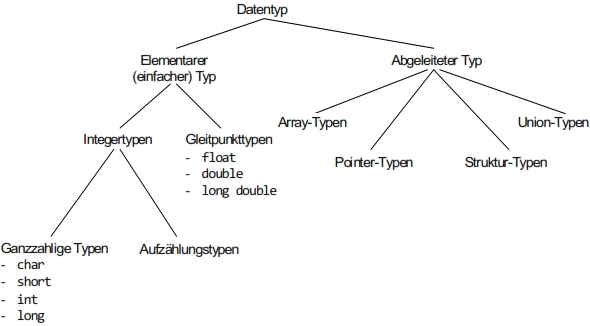
\includegraphics[width=1\textwidth]{pics/datentypen_klassifikation.jpg}
		\end{minipage}
		%
		\begin{minipage}[c]{10 cm}
			In der Programmiersprache C gibt es drei Klassen von Typen:
			\begin{compactitem}
				\item Objekttypen (Datentypen): Objekttypen beschreiben Variablen, \\
				z.B. $int$
				\item Funktionstypen: Funktionstypen beschreiben Funktionen, \\
				z.B. $int$ $f$ $(void)$
				\item unvollständige Typen: Der Typ $void$ ist ein unvollständiger Typ, der nicht vollständig gemacht werden kann. Er bezeichnet eine leere Menge und wird beispielsweise verwendet, wenn eine Funktion keinen Rückgabewert oder keine Übergabeparameter hat.
			\end{compactitem}
		\end{minipage}